\documentclass{article}
\usepackage{enumitem}
\usepackage{graphicx}
\usepackage{microtype}
\usepackage{amsmath}
\usepackage[utf8]{inputenc}
\newcommand{\myskip}{\par\null\par}
\title{Math 305 Homework 3}
\author{Theodore Koss}
\date{March 2023}
\begin{document}

\maketitle

\section*{Section 3: Solving systems of differential equations}
\subsection*{Exercise 3.1}
\begin{itemize}
    \item $v_0=(50,500)$:\newline 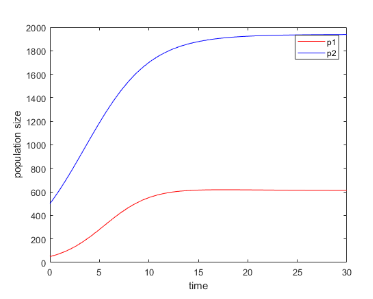
\includegraphics[scale=.6]{Pictures/Pic6.png}
    \item $v_0=(500,50)$:\newline 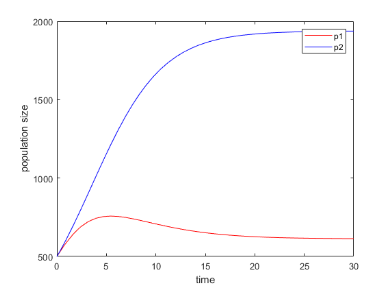
\includegraphics[scale=.6]{Pictures/Pic7.png}
    \item $v_0=(1,1)$:\newline 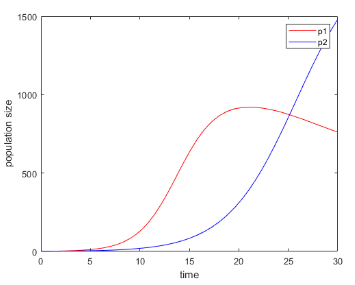
\includegraphics[scale=.6]{Pictures/Pic8.png}
\end{itemize}
\begin{itemize}
    \item The long-term behaviour of the populations do not change.
    \item $P_1$ and $P_2$ do not converge unless the first term of $v(0)$ is greater than the second. I.e, $P_1$ starts higher than $P_2$.
\end{itemize}
\subsection*{Exercise 3.2}
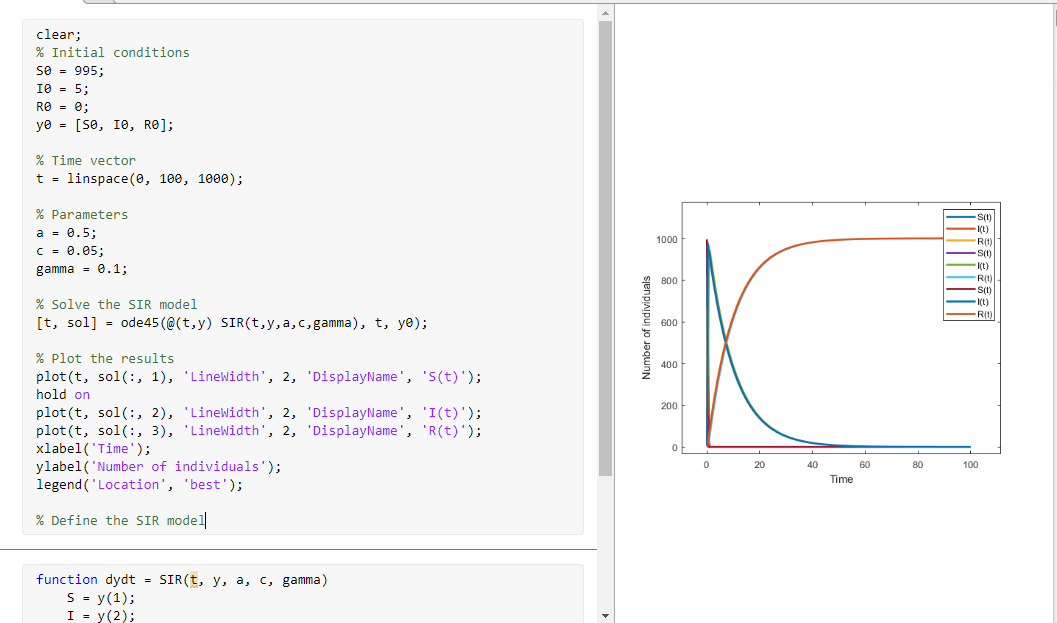
\includegraphics[scale=.3]{Pictures/Pic4.png}\newline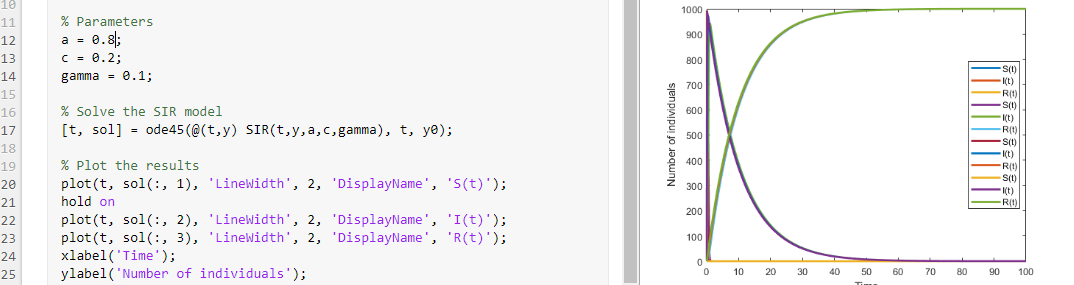
\includegraphics[scale=.3]{Pictures/Pic5.png}\myskip The relationship between $a,c,$ and $\gamma$ to prevent an epidemic must be $ac<\gamma$. This can be achieved by increasing gamma, or decreasing $a$ or $c$. Decreasing the rate of transmission ($a$) or the proportion of susceptible individuals who come into contact with infectious individuals ($c$), will reduce the chance of an epidemic. Increasing the recovery rate ($\gamma$) will also reduce the chance of an epidemic.
\subsection*{Problem 3}Diana is a 160-lb woman who consumes five standard glasses of wine in a short amount of time.\begin{enumerate}[label=(\alph*)]
    \item Estimate her BAC. $BAC = (A\cdot 5.14 / W \cdot r) - 0.015\cdot H$, assuming she drank 5 5oz glasses in 1 hr: $$BAC=(25\cdot5.14/160\cdot0.55) - 0.015=0.1185$$ 
    \item Use the Widmark model to estimate how long it will take before Diana is legally able to drive. Solving for $H$: $$H = (A \cdot 5.14 / W\cdot r - BAC) / 0.015$$ Legal BAC is .08, so plugging in: $$H = (25\cdot 5.14 / 160\cdot0.55 - 0.08) / 0.015=3.36\ \mathrm{hours}$$
    \item Use the Wagner model simulation to estimate how long it will take before Diana is legally able to drive.\newline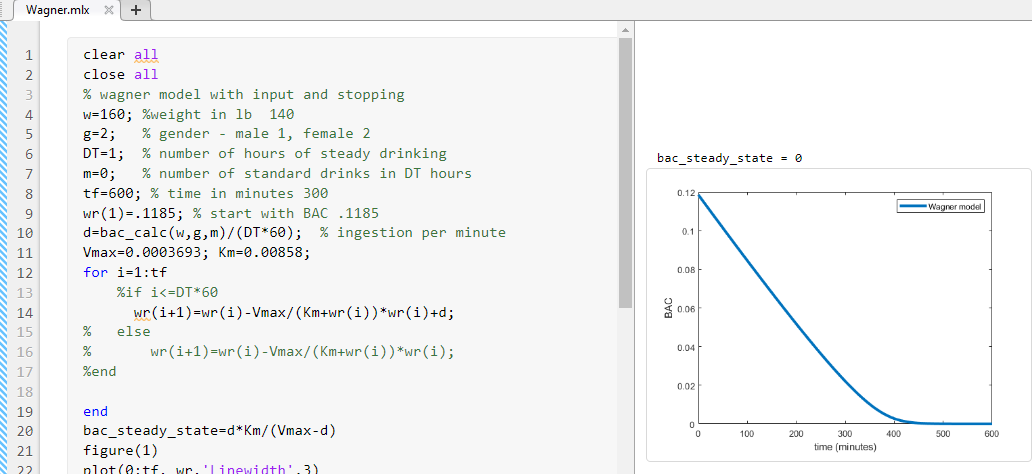
\includegraphics[scale=.4]{Pictures/Pic9.png}\myskip About 1 hour and 55 minutes, $t=115$ minutes.
\end{enumerate}
\end{document}